\chapter{System Build and Estimation}
\label{ch:estimate}

The controllers of Chapter~\ref{ch:design} need a machine that can produce their signals and a numerical procedure that can score them without pretending to be a field season. Section~\ref{sec:build} specifies that machine as a system build: mechanics only so far as the signals require, then sensors, computers, timing, and calibration. Section~\ref{sec:estimation} integrates the same models the controllers use and reads the indices defined in Section~\ref{sec:problem}.

\section{System build}
\label{sec:build}

\subsection{What the build is for}

The build is a single-row wooden-seed planter whose information architecture matches Figure~\ref{fig:hierarchy}. It is specified here as an engineering description, not as a fabricated prototype. No mass, no weld, and no photographed assembly is claimed. The description is detailed because a control design that does not name its sensors cannot be implemented, and because several modelling assumptions in Chapter~\ref{ch:design} are assumptions about hardware. The isolator attenuation $\alpha_{\mathrm{iso}}=0.55$, the depth-noise reduction from 6.5~mm to 1.2~mm, and the refusal to take speed from a driven wheel are all build decisions. If a later prototype changes them, the estimation has to be rerun. That dependency is intentional.

The agronomic envelope is the one already used in the hardwood trials and in the direct-seeding review. Forward speed is 0.6 to 1.2~m/s. Target spacing is 0.25~m, which is a restoration spacing rather than a nursery-bed spacing of several seeds per foot \cite{dinkel1991,lof2019}. Target depth is 30~mm, inside the band in which acorns are covered without being buried past their reserves. The cell mouth is 24~mm, chosen as a compromise around red oak and knowingly wrong for pin oak and bur oak. The control system is the means of living with that compromise. A family of interchangeable cells would also work, and would not need this thesis. The build keeps one cell in order to force the controllers to do the work.

\subsection{Mechanical path of a seed}

Seeds sit in a hopper of about 15~litres, enough for a short bout at 4.4~seeds/s without a refill and small enough that the changing head of seeds is a real load disturbance on the wheel. The hopper floor is a short vibratory tray driven by an electromagnetic shaker. The tray discharges into a throat that is the camera's window. Below the window, a 12-cell wheel of 180~mm pitch diameter picks seeds from the throat and carries them to a release at the bottom of the housing. Elastomer inserts in the cells accept a diameter band around 24~mm without machining a new wheel for each species. They do not, and cannot, accept a 32~mm acorn and a 15~mm acorn with equal fill. That is the residual the controllers are scored on.

A low-pressure port opens onto the cell during the rising half of the rotation and is vented before release. The port is the assist vacuum. Its regulator must be able to hold 0~kPa, meaning the port is open to atmosphere, because the cost will select that point for small seeds. A regulator that cannot go to zero is the wrong part, even if its span is otherwise impressive. The maximum used by the grid is 5~kPa, and the hardware stop is 8~kPa, above the grid so that a faulted command still has a relief valve under the cereal pressures that this machine deliberately does not use \cite{karayel2004,li2025drum}.

From the release, a smooth tube of 40~mm inside diameter drops the seed to the opener. The tube is straight enough that a photoelectric gate sees one chord of the seed, and short enough that time of flight at a drop of 0.4~m is under 0.3~s. That delay is why the gate is a logger and not the bridge sensor. The opener is a narrow shoe behind a ripper point, the arrangement Wells adopted after a plain no-till opener failed to penetrate spoil \cite{wells1990}. Depth is set by a linear actuator against a gauge wheel, with a potentiometer on the pivot. A press wheel closes the slot. The press wheel is not controlled. Its load is a spring.

The vibratory tray, the cell wheel, the vacuum port, and the opener are the four actuated elements. Everything else is structure. The structure that matters to the model is the mount between the seed box and the frame. Rubber isolators are specified at the box feet, and the coordinator-on case takes their attenuation of terrain frequency as $\alpha_{\mathrm{iso}}=0.55$ in Equation~\eqref{eq:feff}. The coordinator-off case bypasses the assumption by using $\alpha_{\mathrm{iso}}=1$, which represents either locked mounts or a frame that was never isolated. This is a coarse representation of a transfer function. It is enough to let the cost discover that adding shaker frequency on top of an already harsh frame is expensive in misses. A measured transmissibility would replace the constant 0.55 without a change to the grid search.

\begin{figure}[htbp]
\centering
\begin{tikzpicture}[
  font=\scriptsize,
  box/.style={draw, rounded corners=1pt, align=center, inner sep=2pt},
  arr/.style={-{Stealth[length=1.8mm]}, thin}
]
\draw[thick] (0,0) rectangle (14.2,4.6);
\node[box, minimum width=22mm] at (1.7,3.6) {Hopper};
\node[box, minimum width=22mm] at (1.7,2.5) {Shaker tray\\$f$};
\node[box, minimum width=24mm] at (4.6,2.5) {Throat window\\camera};
\node[box, minimum width=22mm] at (7.4,2.5) {12-cell wheel\\$\omega$, vacuum $P$};
\node[box, minimum width=18mm] at (9.8,1.5) {Tube and\\light gate};
\node[box, minimum width=22mm] at (12.2,1.5) {Opener\\depth $h$};
\draw[arr] (1.7,3.2) -- (1.7,2.9);
\draw[arr] (2.8,2.5) -- (3.5,2.5);
\draw[arr] (5.7,2.5) -- (6.4,2.5);
\draw[arr] (8.4,2.2) -- (9.2,1.8);
\draw[arr] (10.7,1.5) -- (11.2,1.5);
\node[align=left] at (4.2,0.7) {Isolated box mount, $\alpha_{\mathrm{iso}}$};
\node[align=left] at (11.2,0.7) {Gauge wheel and press wheel};
\node[align=left, anchor=west] at (0.3,4.2) {Single row, 0.6--1.2~m/s, $X_t=0.25$~m};
\end{tikzpicture}
\caption{Seed path assumed by the controllers. Only frequency, vacuum, wheel speed, and depth are commands. The light gate counts seeds after release.}
\label{fig:machine}
\end{figure}

\subsection{Sensor list and what each signal is allowed to do}

Table~\ref{tab:sensors} is the interface control document in miniature. A signal that is not in the table does not enter a control law in this design. Adding a signal later is a revision, not a silent improvement, because the estimation will not have seen it.

\begin{table}[htbp]
\centering
\caption{Sensors, rates, and the loop allowed to consume each signal.}
\label{tab:sensors}
\begin{tabular}{@{}p{32mm}p{22mm}p{28mm}p{55mm}@{}}
\toprule
Sensor & Period & Consumer & Use \\
\midrule
Radar or undriven-wheel encoder & 10~ms & Feed loop & Ground speed $v$ in the kinematic law \\
Cell-wheel encoder & 10~ms & Feed loop & Shaft speed $\omega$ for the fuzzy PID \\
Throat camera & 50~ms & Vision computer & Features $\bar d$, $c_d$, $\rho$, $B$ \\
Tube light gate & event & Logger only & Delivered-rate estimate, not the constraint \\
Opener potentiometer & 10~ms & Depth servo & Hold $h^{\star}=30$~mm \\
Inertial unit on the frame & 20~ms & Factor loop & Dominant terrain frequency $f_{\mathrm{dist}}$ \\
Shaker current & 10~ms & Shaker amplifier & Track the frequency command \\
Vacuum transducer & 20~ms & Regulator & Track $P$, including the zero point \\
Hopper load cell & 100~ms & Logger only & Refill warning below 15 percent mass \\
\bottomrule
\end{tabular}
\end{table}

The inertial unit is not a navigation system. A short Fourier magnitude, updated every 200~ms on a one-second window of vertical acceleration, supplies the peak frequency inside 2 to 30~Hz. That peak is $f_{\mathrm{dist}}$ in Equation~\eqref{eq:feff}. If the spectrum is flat, the factor loop uses the last peak and sets a stale flag. A stale disturbance frequency freezes the frequency command and still allows vacuum to be optimised, because vacuum does not depend on $f_{\mathrm{eff}}$ except through the shared cost.

The camera calibration is a scale factor from pixels to millimetres, obtained from a 20~mm disk placed in the throat. Equivalent diameter in Equation~\eqref{eq:deq} inherits that scale. A 5 percent scale error moves a 20~mm seed by 1~mm, which is small beside the gap between pin oak and bur oak and is large beside a claim of millimetre metrology. The design does not make a millimetre claim. It claims that the bridge index rank-orders a packed throat against a flowing one.

\subsection{Computers and the bus between them}

Two processors are specified, matching the deadline split.

The feed computer is a small microcontroller with a hardware encoder interface and a 10~ms timer interrupt that cannot be disabled by the communication routine. It runs Equation~\eqref{eq:pid} and Equation~\eqref{eq:sigma}. It receives feature datagrams and factor-health bits. It does not decode images. Its worst-case execution for the control step is required to be under 2~ms, leaving 8~ms of idle time inside the period. That idle time is the margin Borja's combined processor did not have \cite{borja2021}.

The vision and factor computer is a single-board processor with a camera interface. Vision and the grid search share it because both are slow relative to the motor and both tolerate a missed deadline. They do not share a thread. Vision is a high-priority periodic thread at 50~ms. The grid search is a lower-priority thread released every 200~ms. If the search is still running when the next vision frame is due, the frame runs and the search continues. If the search is still running at the next 200~ms boundary, its result is discarded and the previous $(f,P)$ is held. Discarding a late result is safer than applying a result computed from a stale $\bar d$ that has since been replaced. The search was sized at 55 costs so that a discard is a fault, not the normal path.

The datagram between the boards is a fixed 32-byte record: time stamp, $\bar d$, $c_d$, $\rho$, $B$, vision-health, factor-health, $f$, $P$, and a checksum. A failed checksum is treated as a missed vision frame and follows the hold-and-decay rule. There is no dynamic allocation in the receive path. An ISO~11783 implement bus can carry the spacing set-point $X_t$ from a tractor terminal in a later integration \cite{iso11783}. The control laws do not read that bus in the design scored here. $X_t$ is a stored parameter.

Power is a 12~V machine bus with a separate regulator for the cameras and processors, so that a shaker current spike does not brown out the microcontroller. The shaker amplifier and the wheel motor have their own drivers and their own current limits. The wheel-motor current limit is set so that a jammed cell stalls the motor and raises the encoder-loss fault, rather than shearing the elastomer. That current limit is a mechanical-protection setting. It is not a control gain.

\subsection{Software tasks}

The tasks and their budgets are listed in Table~\ref{tab:tasks}. Budgets are requirements on a future implementation. They are consistent with the periods in Table~\ref{tab:params}. They have not been measured on a board in this study.

\begin{table}[htbp]
\centering
\caption{Tasks, periods, and the action on a missed deadline.}
\label{tab:tasks}
\begin{tabular}{@{}p{38mm}p{18mm}p{28mm}p{58mm}@{}}
\toprule
Task & Period & Budget & On a missed deadline \\
\midrule
Motor control & 10~ms & 2~ms & Stop the wheel if two periods are missed \\
Vision features & 50~ms & 30~ms & Feed loop holds $B$, then decays it \\
Depth servo & 10~ms & 1~ms & Hold last valve or motor command for 50~ms, then freeze depth \\
Disturbance spectrum & 200~ms & 20~ms & Freeze $f$, continue vacuum search \\
Factor grid & 200~ms & 40~ms & Keep previous feasible $(f,P)$ \\
Logger & 100~ms & 10~ms & Drop the oldest log block \\
\bottomrule
\end{tabular}
\end{table}

The logger is the only task allowed to drop data. Control tasks hold a feasible command or they stop the actuator. This is the operational content of requirement~9 in Section~\ref{sec:problem}. It is also the reason the factor search was not placed inside the motor interrupt. An occasional 40~ms search is acceptable on its own core and unacceptable inside a 10~ms interrupt.

State machines for the feed faults were listed in Section~\ref{sec:visiondesign}. The factor task adds two states. In \emph{search}, it publishes a new grid minimiser after the slew limit. In \emph{hold}, it publishes the previous command and lights a lamp. Entry to \emph{hold} is a late search, a stale $\bar d$ older than 500~ms, or a wheel-stopped bit from the feed computer. Exit from \emph{hold} requires three healthy cycles, so a flickering health bit does not chatter the shaker.

\subsection{Calibration procedure}

Calibration is a procedure, not a learning algorithm. It is specified because the features and the depth servo are meaningless without it. The order matters. A scale factor computed before the camera is clamped will be repeated after the next service and will silently shift $B$.

\begin{enumerate}
\item Clamp the camera and the lamp. Place the 20~mm disk in the throat on the centreline. Record the equivalent diameter reported by Equation~\eqref{eq:deq} and set the millimetre scale so that the report is 20~mm. Repeat at 10~mm left and right of centre. Reject the mount if the three reports differ by more than 0.6~mm.
\item Empty the throat. Record the residual image used by the background subtraction. Confirm that occupancy reads below 0.02.
\item Command the wheel at 15~r/min with an empty throat. The shaft encoder and a hand tachometer shall agree within 0.3~r/min. This checks Equation~\eqref{eq:wstar2}'s sensor, not the seed path.
\item Command $f$ from 2 to 12~Hz in 2~Hz steps against a strobe or a frequency output of the amplifier. The inertial unit, mounted for this step on the tray rather than on the frame, shall report the same peak within 0.5~Hz. Then return the unit to the frame.
\item Command $P$ at 0, 2, and 5~kPa. The transducer shall read within 0.3~kPa. The zero command shall read below 0.2~kPa. A zero that actually holds 1~kPa will bias the cost toward doubles on small seeds.
\item Set the opener on a flat rail and command 20, 30, and 40~mm. The potentiometer reading shall be within 1.5~mm. This is the sensor error. The 1.2~mm standard deviation used in the estimation is the closed-loop residual about the set-point, which includes rail roughness in the model and is not the same number as the calibration tolerance.
\item Drive the unit on a hard surface at a constant 1.0~m/s and compare radar speed with distance over time. The mean error shall be below 2 percent. Slip of a driven wheel is not a failure of this check. A difference between radar and the driven wheel is the slip the control law is there to ignore.
\end{enumerate}

No seed is required for these steps. A seed check is a bench experiment and sits outside this manuscript. The estimation does not use the tolerances as random errors except for the depth residual and the slip model already stated. Adding the calibration tolerances as extra noise would be a straightforward sensitivity run. It was not the run reported below.

\subsection{Safety interlocks}

The wheel motor is disabled when the opener is raised, so that a headland turn does not drill seeds onto the surface. The shaker is disabled when the hopper mass is below the refill threshold, so that an empty tray is not driven at 10~Hz for a bout. The vacuum pump or regulator is disabled at the same time. These interlocks are combinational logic on the feed computer, independent of the factor search. A software fault in $J$ cannot leave the shaker running on an empty machine once the load cell has crossed the threshold. The load cell itself can fail. A stuck high reading leaves the shaker enabled, which is the worse direction for noise and the safer direction for not silencing a full hopper. The failure is detected by the operator from the mass display, not by a second estimator.

\section{Estimation}
\label{sec:estimation}

\subsection{What is being estimated}

The estimation integrates the event model of Section~\ref{sec:predmodel} over long sequences of seeds. It asks how the indices move when the feed law and the factor law are switched on and off. The plant and the coordinator's predictor are the same logistic map. The Monte Carlo still has private randomness: each event draws a diameter from the lot, a slip, and a depth error. The coordinator sees only the lot mean and coefficient of variation. The feed constraint sees a filtered occupancy state, not the next diameter. The comparison is therefore a comparison of information and of actions, not a replay of one open-loop trajectory.

Five modes are defined.

\begin{enumerate}
\item \textbf{Ground.} The wheel is geared to the driven wheel. The speed scale equals $1-s$. Slip has mean $0.07+0.012$ times slope in degrees. Factors are fixed at $f=0$, $P=3$~kPa, and a passive depth error of standard deviation 6.5~mm. Terrain enters with $\alpha_{\mathrm{iso}}=1$.
\item \textbf{PID.} Electronic tracking of $\omega^{\star}$ from radar speed. The scale is 1 plus a small tracking residual of standard deviation 0.012. No vision constraint. Factors remain at the ground-drive constants. Slip is rejected except for a quarter of the ground-drive slip passed into the probability map, representing residual speed error.
\item \textbf{Vision.} The PID mode plus the bridge constraint of Equation~\eqref{eq:sigma}. Factors remain fixed. This mode is the first innovation alone.
\item \textbf{MPC.} The PID mode plus the grid minimiser of Equation~\eqref{eq:cost}, the isolated mount $\alpha_{\mathrm{iso}}=0.55$, and the tight depth residual of standard deviation 1.2~mm. Vision is off. This mode is the second innovation alone.
\item \textbf{Both.} Vision and MPC together.
\end{enumerate}

Each case runs 4{,}000 cell events. The random generator is the NumPy generator with seed 20261029 for the main table, and with seeds $20261029+17r$ for twelve repeats of the mixed-lot gain. The script that implements the modes is \texttt{simulate\_estimation.py}, stored with this manuscript. A reimplementation that follows Section~\ref{sec:predmodel} and the mode list above should match the table to sampling error. The script is the definition of the sampling error that was actually used.

Lots are log-normal in diameter. Pin oak has mean 15~mm and coefficient of variation 0.12. Red oak has 20.5~mm and 0.15. Bur oak has 32~mm and 0.20. The mixed lot has 22~mm and 0.32, which is a stand-in for a hopper that was not cleaned between species. Scenarios cross these lots with speed, slope, and a terrain frequency. The eight scenarios are the rows of the tables in this section. They were chosen to probe the requirements: a mild red-oak baseline, a slope, a harsh vibration, a small seed, a large seed, and a mixture.

Indices follow Equations~\eqref{eq:imult}--\eqref{eq:eta}. Positions are accumulated by advancing $X_t/\sigma$ at each event, placing one seed on a single, placing two seeds 0.22$X_t$ apart on a double, and placing nothing on a miss. Scatter from Equation~\eqref{eq:sigma_scatter} is added to the placed positions. Spacings are the positive differences of the sorted positions. This construction is how a miss becomes a gap near $2X_t$ and a double becomes a short gap, which is what the Kachman indices count \cite{kachman1995,iso7256}.

\subsection{Mild red oak}

Table~\ref{tab:redmild} gives red oak at 1.10~m/s, no slope, and a 6~Hz terrain disturbance. This is the easiest hardwood case that is still not a maize case. The cell is only slightly large for the seed.

\begin{table}[htbp]
\centering
\caption{Red oak, $v=1.10$~m/s, level ground, terrain frequency 6~Hz. Energy is the mean per event of $0.08\omega^2+0.012 f^2+0.02 P^2$ in the units of the script.}
\label{tab:redmild}
\begin{tabular}{@{}lrrrrrrr@{}}
\toprule
Mode & $Q_{\mathrm{f}}$ & $I_{\mathrm{mult}}$ & $I_{\mathrm{miss}}$ & $C_{\mathrm{v}}$ & $\eta_{\mathrm{E}}$ & Energy \\
\midrule
Ground & 58.58 & 21.65 & 19.78 & 20.13 & 52.38 & 0.55 \\
PID & 60.89 & 22.50 & 16.61 & 21.20 & 60.97 & 0.60 \\
Vision & 68.51 & 12.52 & 18.97 & 17.85 & 60.70 & 0.60 \\
MPC & 77.11 & 11.96 & 10.93 & 16.00 & 76.56 & 1.40 \\
Both & 88.20 & 5.59 & 6.22 & 12.88 & 87.00 & 1.39 \\
\bottomrule
\end{tabular}
\end{table}

Reading down the table is the answer to the three research questions for this scenario. The PID mode, which only rejects slip, moves the miss index from 19.8 to 16.6 percent and moves efficiency from 52.4 to 61.0 percent. It does nothing for doubles. The multiple index stays near 22 percent because the fixed 3~kPa vacuum and the slightly large cell are still there. Vision cuts the multiple index from 22.5 to 12.5 percent and raises quality of feed from 60.9 to 68.5 percent. Efficiency does not follow. It stays at 60.7 percent, because some of the seeds that are no longer doubled become stretched spacings and are counted as misses. The miss index rises from 16.6 to 19.0 percent. That rise is the interference the problem statement asked to be kept visible. On this mild case it cancels the productivity gain of vision and leaves the quality gain.

The factor coordinator is the large step. With vision still off, quality of feed reaches 77.1 percent, the miss index falls to 10.9 percent, and efficiency reaches 76.6 percent. The grid selects $f=9$~Hz and $P=0$. Zero vacuum is the map refusing the cereal habit. Nine hertz is the preferred agitation for a 20.5~mm seed, and with isolation the effective frequency stays under the 10~Hz anchor. Energy rises from 0.60 to 1.40 because the shaker is doing the work the vacuum is no longer doing. Stacking vision on top of that regime cuts the multiple index further, from 12.0 to 5.6 percent, and cuts the miss index as well, from 10.9 to 6.2 percent. Efficiency reaches 87.0 percent. On a regime the coordinator has already made flow, the constraint is active less often in a damaging way, and the two loops agree. Precision stays between 13 and 21 percent in every mode, inside the 30 percent band. Precision is not the term that separates these designs. Misses and doubles are.

The same lot at 0.70~m/s, still level, still at 6~Hz, is close to the 1.10~m/s table. Ground-drive quality of feed is 58.0 percent and efficiency is 51.5 percent. Both-mode quality of feed is 88.2 percent and efficiency is 87.3 percent. Speed, inside this narrow band, is not the main effect. Liu and colleagues found a clear speed effect on maize meters at field speeds well above this band \cite{liu2017speed}. The model does not add a further speed penalty beyond the scale error, so it should not be cited as a prediction of high-speed hardwood planting. The machine was never specified for that speed.

\begin{figure}[htbp]
\centering
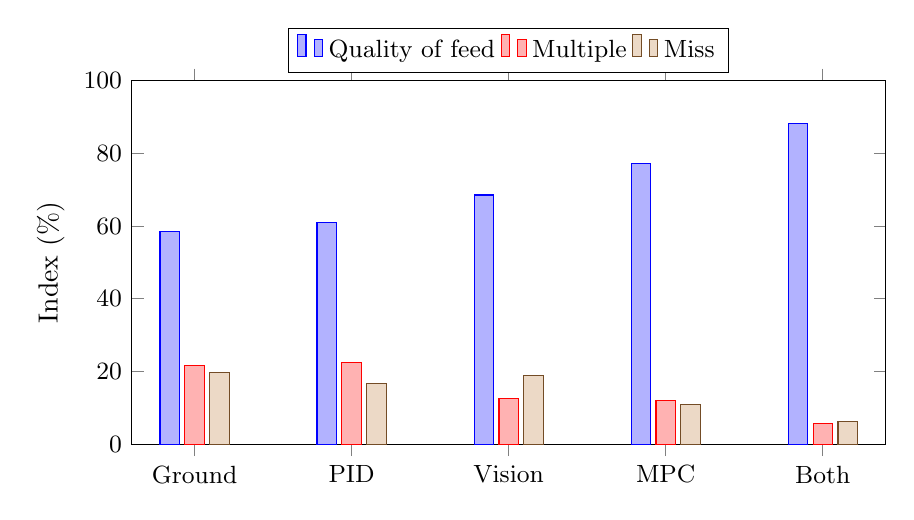
\begin{tikzpicture}
\begin{axis}[
  width=0.92\textwidth, height=6.2cm,
  ybar, bar width=7pt,
  ylabel={Index (\%)},
  symbolic x coords={Ground,PID,Vision,MPC,Both},
  xtick=data,
  ymin=0, ymax=100,
  legend style={font=\small, at={(0.5,1.02)}, anchor=south, legend columns=3},
  tick label style={font=\small}
]
\addplot coordinates {(Ground,58.58) (PID,60.89) (Vision,68.51) (MPC,77.11) (Both,88.20)};
\addplot coordinates {(Ground,21.65) (PID,22.50) (Vision,12.52) (MPC,11.96) (Both,5.59)};
\addplot coordinates {(Ground,19.78) (PID,16.61) (Vision,18.97) (MPC,10.93) (Both,6.22)};
\legend{Quality of feed, Multiple, Miss}
\end{axis}
\end{tikzpicture}
\caption{Red oak on level ground at 1.10~m/s. Vision trades a lower multiple index against a slightly higher miss index. The stacked system lowers both.}
\label{fig:redbars}
\end{figure}

\subsection{Slope and harsh vibration on red oak}

Slope is where the electronic drive earns its keep and where vision adds little. At 1.10~m/s and 12 degrees, with terrain still at 6~Hz, ground-drive quality of feed falls to 46.3 percent and efficiency falls to 28.9 percent. The miss index is 32.8 percent. Slip has stretched the spacing and the probability map has added misses. The PID mode returns the row to the level-ground electronic result: quality of feed 60.6 percent, efficiency 60.5 percent, miss index 17.2 percent. Vision reaches 68.5 percent quality of feed. MPC reaches 77.3 percent. Both reaches 88.2 percent quality of feed and 87.1 percent efficiency. Once slip is removed, the slope case and the level case are the same case. That is a property of the model, because slope enters only through slip. A real opener would also see a change of draft on a slope. The build logs draft and does not control it. The estimation therefore has nothing honest to add about draft.

Harsh vibration is a different disturbance. Table~\ref{tab:harsh} raises the terrain frequency to 16~Hz on level ground at 1.10~m/s, still with red oak.

\begin{table}[htbp]
\centering
\caption{Red oak, $v=1.10$~m/s, level ground, terrain frequency 16~Hz.}
\label{tab:harsh}
\begin{tabular}{@{}lrrrrrr@{}}
\toprule
Mode & $Q_{\mathrm{f}}$ & $I_{\mathrm{mult}}$ & $I_{\mathrm{miss}}$ & $C_{\mathrm{v}}$ & $\eta_{\mathrm{E}}$ & $f$ (Hz) \\
\midrule
Ground & 34.47 & 20.94 & 44.59 & 22.64 & 17.11 & 0 \\
PID & 36.94 & 21.20 & 41.86 & 24.24 & 21.77 & 0 \\
Vision & 41.12 & 13.24 & 45.64 & 21.89 & 21.99 & 0 \\
MPC & 67.16 & 16.28 & 16.56 & 18.80 & 64.46 & 3 \\
Both & 72.68 & 9.70 & 17.62 & 16.11 & 64.28 & 3 \\
\bottomrule
\end{tabular}
\end{table}

Shaft-speed tracking barely moves the miss index, from 44.6 to 41.9 percent. The seeds are being shaken out of the fill, and the shaft is not the cause. Vision lowers doubles from 21.2 to 13.2 percent and raises misses from 41.9 to 45.6 percent. Efficiency stays near 22 percent. Slowing a meter that is already missing because of vibration creates longer gaps. This is the clearest negative result for the first innovation used alone. It matches the design warning: the constraint is not a substitute for a bad factor regime.

The coordinator drops the shaker command from the 9~Hz of the mild case to 3~Hz. With $\alpha_{\mathrm{iso}}=0.55$, a 16~Hz terrain contribution and a 3~Hz command give an effective frequency near $\sqrt{(0.55\cdot 16)^2+3^2}\approx 9.3$~Hz, just under the harshness anchor. The miss index falls to 16.6 percent and efficiency rises to 64.5 percent. Energy per event falls to 0.53, below the PID mode's 0.60, because the optimiser has chosen the quiet command. Stacking vision raises quality of feed from 67.2 to 72.7 percent and cuts doubles from 16.3 to 9.7 percent, but efficiency does not rise. It is 64.3 percent. The extra quality is real and the extra planting rate is not, because the constraint still stretches some spacings. A user who cares about $Q_{\mathrm{f}}$ turns both loops on. A user who cares only about $\eta_{\mathrm{E}}$ under a 16~Hz disturbance gets essentially the whole gain from the factor loop and the isolator.

The 3~Hz choice is not a rule written for 16~Hz. It is the grid minimum of Equation~\eqref{eq:cost}. Neighbouring commands at 2~Hz and 4~Hz were available and lost. This is the behaviour required by requirement~8.

\subsection{Pin oak and the multiple index}

Pin oak at 15~mm is the small-seed requirement. At 1.10~m/s, level, 6~Hz terrain, ground drive posts a multiple index of 33.7 percent, a miss index of 15.7 percent, and a quality of feed of 50.6 percent. The cell is simply large. PID tracking leaves the multiple index at 34.3 percent and raises efficiency from 54.9 to 61.6 percent by removing slip. Vision cuts multiples to 24.3 percent and raises quality of feed to 60.6 percent. Efficiency moves only to 63.8 percent. The first innovation helps, and it does not repair a 9~mm mismatch by itself.

The coordinator selects 10~Hz and again 0~kPa. Quality of feed rises to 70.0 percent and the multiple index falls to 19.4 percent. Both loops together reach a multiple index of 10.3 percent, a miss index of 6.3 percent, a quality of feed of 83.4 percent, and an efficiency of 86.5 percent. The stack is worth more here than it was under harsh vibration. Small seeds double because of geometry and vacuum. Vision sees the irregular occupancy that goes with doubles, and the coordinator has removed the vacuum that was causing them. Each loop's action is aimed at the same error, so they add.

Ten hertz is at the top of the preferred-frequency curve for a 15~mm seed after the clip at 11~Hz. The cost is willing to sit next to the harshness anchor when the terrain itself is only 6~Hz and isolation is on. It is not willing to add 16~kPa, or 50~Hz, which is the vegetable-seed operating point \cite{li2025drum}. The grid's upper pressure is 5~kPa and the optimum is 0. Within the model, assist vacuum is the wrong tool for this cell and this lot.

\subsection{Bur oak and the miss index}

Bur oak is the Wells failure mode, put into the same table as the other lots \cite{wells1990}. The mean diameter is 32~mm against a 24~mm cell. No controller grows the cell. The question is how much of the miss index is recovered by time and by agitation.

At 0.70~m/s, level, 6~Hz, ground drive has a quality of feed of 34.5 percent, a miss index of 52.3 percent, and an efficiency of 14.8 percent. PID moves these to 37.2, 50.3, and 18.4. Vision moves quality of feed to 40.7 percent and efficiency to 16.9 percent, with the miss index still at 53.5 percent. Slowing the wheel without a better fill does not place large seeds. It waits longer between failures.

The coordinator selects 8~Hz and 0~kPa. Quality of feed rises to 63.1 percent, the miss index falls to 30.0 percent, and efficiency rises to 45.6 percent. Both loops reach 76.9 percent quality of feed, a miss index of 19.8 percent, a multiple index of 3.3 percent, and an efficiency of 57.9 percent. The residual miss index near 20 percent is the honest limit of a 24~mm cell on a 32~mm seed inside this map. The design does not claim a maize-grade meter on bur oak. It claims a large recovery relative to ground drive, and the table supports that claim inside the model: the miss index is cut by more than half, and efficiency rises from 15 percent to 58 percent.

The harsher bur-oak scenario adds an 8 degree slope and a 12~Hz terrain frequency at 1.10~m/s. Ground drive collapses to a quality of feed of 20.7 percent, a miss index of 66.5 percent, and an efficiency of 5.0 percent. PID recovers efficiency only to 11.9 percent. Vision, alone, sits at 9.8 percent efficiency with a miss index of 64.1 percent. MPC reaches 61.3 percent quality of feed and 44.0 percent efficiency at 7~Hz and 0~kPa. Both reaches 75.4 percent quality of feed, a miss index of 21.5 percent, and an efficiency of 55.1 percent. The first innovation is not useless in the stack. It is useless as a remedy for this disturbance by itself. That sentence is the practical output of the estimation for an implementer who might otherwise ship the camera and leave the shaker at the factory setting.

\begin{figure}[htbp]
\centering
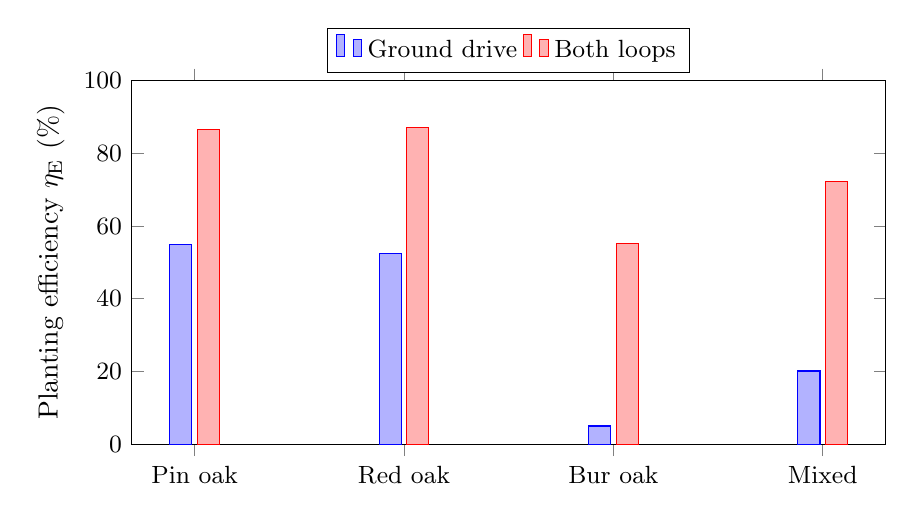
\begin{tikzpicture}
\begin{axis}[
  width=0.92\textwidth, height=6.2cm,
  ybar, bar width=8pt,
  ylabel={Planting efficiency $\eta_{\mathrm{E}}$ (\%)},
  symbolic x coords={Pin oak, Red oak, Bur oak, Mixed},
  xtick=data,
  ymin=0, ymax=100,
  legend style={font=\small, at={(0.5,1.02)}, anchor=south, legend columns=2},
  tick label style={font=\small},
  x tick label style={font=\small}
]
\addplot coordinates {(Pin oak,54.87) (Red oak,52.38) (Bur oak,5.01) (Mixed,20.12)};
\addplot coordinates {(Pin oak,86.49) (Red oak,87.00) (Bur oak,55.12) (Mixed,72.25)};
\legend{Ground drive, Both loops}
\end{axis}
\end{tikzpicture}
\caption{Planting efficiency of ground drive against both loops. Pin oak and red oak are the mild electronic cases at 1.10~m/s. Bur oak and the mixed lot include slope and a terrain frequency of 12~Hz. The bur-oak bar remains the lowest of the stacked results, which is the large-seed limit of a 24~mm cell.}
\label{fig:compare}
\end{figure}

\subsection{Mixed lot}

The mixed lot combines a 22~mm mean with a coefficient of variation of 0.32, an 8 degree slope, and a 12~Hz disturbance, at 1.10~m/s. It is the scenario in which a single fixed setup is least defensible. Ground drive scores 36.9 percent quality of feed, 24.0 percent multiples, 39.1 percent misses, and 20.1 percent efficiency. PID raises efficiency to 37.8 percent by rejecting slip and leaves multiples at 24.2 percent. Vision raises quality of feed to 50.4 percent, cuts multiples to 14.9 percent, and lowers efficiency to 33.5 percent. Again the constraint improves the composition of errors and gives back part of the rate.

MPC, at 8~Hz and 0~kPa, reaches 68.0 percent quality of feed and 65.2 percent efficiency. Both reaches 80.7 percent quality of feed, 7.6 percent multiples, 11.7 percent misses, precision 13.8 percent, and efficiency 72.3 percent. Twelve repeats of this one scenario, with different generator seeds, give a mean efficiency gain of the stacked system over ground drive of 50.8 percentage points, with a standard deviation of 0.89 points. The gain is stable across draws because 4{,}000 events is a long run. It is not stable across scenarios, and it should not be quoted as a universal 51-point improvement. On mild red oak the efficiency gain is $87.0-52.4=34.6$ points. On harsh red oak it is $64.3-17.1=47.2$ points. On the harsh bur-oak case it is $55.1-5.0=50.1$ points, from a very low base. The mixed-lot repeat only says that Monte Carlo noise is not the source of the ranking.

\subsection{Energy and the price terms}

Energy in the tables is not joules on a named motor. It is the mean per event of $0.08\omega^2 + 0.012 f^2 + 0.02 P^2$, evaluated in the script so that a faster wheel, a faster shaker, and a higher vacuum all cost something. Because the optimum vacuum is zero in every MPC row, the vacuum term does not drive the comparison. The shaker term does. Mild red oak at 9~Hz costs about 1.39 per event in the both-mode, against 0.60 for PID. Harsh red oak at 3~Hz costs 0.53, which is less than PID, because the wheel speed is similar and the shaker is quiet. The prices inside $J$ are what allow that quiet point to win when agitation would push $f_{\mathrm{eff}}$ over 10~Hz. If the prices were removed, the grid could still avoid 10~Hz through the harshness term in $z_m$. The prices matter for ties. They are not the sole reason the harsh-case command falls.

A deployer who is short of electrical power learns a specific lesson. The camera and the fuzzy loop are cheap in this energy proxy. The shaker is the cost of the second innovation, and it is a cost the optimiser already turns down when the frame is doing the shaking. Running the shaker at 9~Hz out of habit during a 16~Hz bout would pay the energy and, inside the model, would also pay in misses.

\subsection{Where the estimation can mislead}

Several readings would be stronger than the evidence.

The plant is the predictor. A coordinator that minimises $J$ on $\Pi$ will look good when the world is $\Pi$. The private randomness prevents a perfect score, and the tables show residual misses above 6 percent even in the best red-oak row, but a systematic error in the sign of a coefficient would move the real machine in the wrong direction while these tables stayed flattering. The coefficients most exposed to that risk are the 10~Hz anchor, which was observed on rapeseed \cite{zhang2024vib,wu2022}, and the isolator constant 0.55, which was not observed at all. A bench measurement of acorn fill against shaker frequency on this cell would replace both the anchor and the Gaussian width in Equation~\eqref{eq:agit}. Until that measurement exists, the ranking is a design calculation.

The camera is not simulated as an image. Occupancy is a filtered state driven by the rule in the script, not by rendered acorns. Occlusion, dust, and strobe failure are absent. The fault logic specifies what the software should do when features stop. It does not estimate how often they stop. Borja's accuracy on a clean plate, a fraction of a percent of frames wrong, is the optimistic reference \cite{borja2021}. A throat of wooden seeds is a harder image than a painted plate hole.

Depth noise is an independent Gaussian. Real depth error is correlated along the row, because the soil is correlated. Correlated error would widen the distribution of local spacing less than the independent model if the opener rides over a long wave, and it would create bursts of misses if the opener dives. The index means might move less than the appearance of a planted row. The estimation reports means.

Germination, rodent take, and the difference between a spacing and a surviving seedling are outside the indices by the scope statement \cite{lof2019,grossnickle2012}. A high $\eta_{\mathrm{E}}$ can still be a poor plantation. The machine-level claim stops at placement.

The ground-drive baseline uses $P=3$~kPa because that is a plausible leftover cereal setting, not because a hardwood manufacturer recommends it. Part of the MPC gain is the removal of a harmful default. If the baseline is redefined as $P=0$ and $f=0$ with electronic speed already on, the remaining gain is agitation, isolation, and depth, plus vision. That comparison is the PID-versus-MPC gap in the tables, not the ground-versus-both gap. On mild red oak it is $87.0-61.0=26.0$ efficiency points, still large, and it does not depend on accusing the ground drive of a bad vacuum. On that reading the PID row already has the bad vacuum. The MPC row removes it. The gain is still the factor decision.

\subsection{Answers to the research questions}

The questions in Section~\ref{sec:problem} can now be answered in the only sense this manuscript supports: as statements about the model.

The feed-speed loop with a vision constraint reduces doubles beyond shaft-speed tracking. On mild red oak the multiple index falls from 22.5 to 12.5 percent. On pin oak it falls from 34.3 to 24.3 percent. The same loop does not, by itself, reduce misses on bur oak or under a 16~Hz disturbance, and it can lower planting efficiency by stretching spacings. The first innovation is a quality intervention with a rate side effect. It should not be sold as a productivity controller.

The factor coordinator improves the indices in the regimes where tracking has little to offer. Under 16~Hz terrain the efficiency index moves from 21.8 percent with PID to 64.5 percent with the coordinator, at a lower shaker command. On harsh bur oak it moves from 11.9 percent to 44.0 percent before vision is added. The coordinator selects zero assist vacuum for every lot in the grid. Within the model, the right vacuum for this cell is none.

The loops interfere when the factor regime is bad, and they reinforce when the regime is good. Interference shows up as a quality gain without an efficiency gain: vision versus PID on mild red oak, and both versus MPC under 16~Hz. Reinforcement shows up as a gain in both indices: both versus MPC on pin oak, on bur oak, and on the mixed lot. The architecture did not make interference impossible. It made interference visible, because the two indices are published separately and because the coordinator is not allowed to assume that vision will hide its mistakes. That visibility is the system result. An implementer can turn the constraint off under a measured high terrain frequency and leave it on for a mixed or small-seed lot, using the same programs.

\subsection{What a bench would have to show}

A minimal bench, if one is built from Section~\ref{sec:build}, would need only enough instrumentation to recompute Table~\ref{tab:redmild} and Table~\ref{tab:harsh}. A sticky belt or a grease belt under the tube, a variable-speed belt under the wheels, and a shaker under the frame would reproduce the five modes \cite{panning2000,onal2009}. The acceptance test is not a single threshold. It is the ranking. Vision should cut the multiple index relative to PID on red oak and on pin oak. Vision alone should not be required to raise efficiency under a frame vibration above 10~Hz. The coordinator should select a low frequency in that case and a higher frequency when the frame is quiet. Both together should beat PID on bur oak by a margin large enough to see in a few hundred seeds, not only in 4{,}000. If the bench reverses the sign of the frequency effect, the Gaussian in Equation~\eqref{eq:agit} is the part to refit. The cascade structure, the deadline split, and the separation of $Q_{\mathrm{f}}$ from $\eta_{\mathrm{E}}$ would remain the parts worth keeping.

Until that belt is run, the numbers in this chapter are an estimate of a design, computed from a map that encodes the published failure modes of hardwood metering, of ground-wheel slip, of high-frequency vibration, and of a vision loop that slows the input of seeds. They are large enough, and consistent enough across lots, to justify the bench. They are not themselves the bench.

\subsection{The runs that were summarised}

Two red-oak runs and the slope run were described in prose so that the main tables would stay readable. They are recorded here at the same precision as Table~\ref{tab:redmild}, because a summary that cannot be checked against the script is not a result. Table~\ref{tab:rest} collects them. The both-mode frequency is 9~Hz and the vacuum is 0 in the slow and slope runs, and 3~Hz and 0 in the harsh run already discussed.

\begin{table}[htbp]
\centering
\caption{Remaining red-oak runs. Speed is in m/s, slope in degrees, terrain frequency in Hz.}
\label{tab:rest}
\begin{tabular}{@{}llrrrrr@{}}
\toprule
Case & Mode & $Q_{\mathrm{f}}$ & $I_{\mathrm{mult}}$ & $I_{\mathrm{miss}}$ & $C_{\mathrm{v}}$ & $\eta_{\mathrm{E}}$ \\
\midrule
0.70~m/s, 0$^\circ$, 6~Hz & Ground & 58.02 & 21.53 & 20.45 & 19.45 & 51.45 \\
 & PID & 60.24 & 21.35 & 18.41 & 21.44 & 59.48 \\
 & Vision & 65.58 & 13.27 & 21.16 & 18.12 & 57.41 \\
 & MPC & 77.49 & 12.09 & 10.42 & 16.11 & 77.68 \\
 & Both & 88.17 & 5.84 & 5.99 & 13.09 & 87.31 \\
\midrule
1.10~m/s, 12$^\circ$, 6~Hz & Ground & 46.34 & 20.87 & 32.79 & 17.57 & 28.89 \\
 & PID & 60.62 & 22.17 & 17.21 & 20.40 & 60.49 \\
 & Vision & 68.46 & 13.43 & 18.11 & 18.11 & 62.01 \\
 & MPC & 77.28 & 11.46 & 11.26 & 16.01 & 75.82 \\
 & Both & 88.22 & 5.61 & 6.17 & 12.57 & 87.05 \\
\bottomrule
\end{tabular}
\end{table}

The slow run repeats the mild-run pattern at a lower shaft speed. Vision lowers the multiple index from 21.4 to 13.3 percent and lowers efficiency from 59.5 to 57.4 percent. The rate side effect is visible even when the machine is already going slowly. MPC then both restore efficiency, to 77.7 and 87.3 percent. Nothing in the slow run suggests that the stack depends on the 1.10~m/s condition.

The slope run is the cleanest demonstration of requirement~2. Ground-drive efficiency is 28.9 percent with a miss index of 32.8 percent. Every electronic mode returns to within about one point of its level-ground efficiency at the same speed. The both-mode efficiency is 87.1 percent on the slope and 87.0 percent on the level. The model has no other slope channel. The table is what that modelling choice looks like when it is not smoothed into a sentence. A field trial in which electronic control failed to recover a slope would be evidence of a channel the model omitted, most likely opener draft, and not evidence that the arithmetic of Table~\ref{tab:rest} was mis-copied.

\subsection{Reading the near-tie under harsh vibration}

Section~\ref{sec:estimation} reported a 3~Hz command for red oak at 16~Hz terrain. The grid slice in Chapter~\ref{ch:design} shows why that command should not be over-interpreted. At the nominal diameter the predicted costs at 3~Hz and at 9~Hz differ by about $0.0001$. The drawn sample mean in the recorded run selected 3~Hz. Plant-side, with $\alpha_{\mathrm{iso}}=0.55$, a 3~Hz command and a 16~Hz terrain give $f_{\mathrm{eff}}\approx 9.3$~Hz, and a 9~Hz command would give about 12.6~Hz. The plant therefore experiences a real difference between the two commands even though the predictor, using the heavier weight 0.35 on $f_{\mathrm{dist}}^2$, scores them almost alike. The run that was printed used 3~Hz. A second run whose sample mean broke the tie the other way would print 9~Hz and would show a higher plant-side harshness. The efficiency gain over PID would remain, because both corners beat a command of 0~Hz, which is the PID and ground setting. The identity of the winning hertz would not remain. That is the correct confidence statement. The coordinator rejects the middle of the frequency range and rejects a non-zero vacuum. It does not, on this cost, identify a unique frequency once the terrain is already harsh.

\subsection{A note on repeatability of the other scenarios}

The twelve-repeat standard deviation of 0.89 points was computed only for the mixed-lot efficiency gain. The other scenarios were single runs of 4{,}000 events. A binomial picture of a proportion near 0.6 with 4{,}000 trials has a standard error near $\sqrt{0.6\cdot 0.4/4000}\approx 0.008$, or 0.8 percentage points, before the dependence among successive spacings is considered. Dependence widens the error. Doubling the binomial picture is a cautious reading: differences of two points in the tables are inside noise, and differences of ten points are not. The vision-versus-PID multiple-index drop on mild red oak is about ten points. The both-versus-ground efficiency gaps are tens of points. The vision-versus-PID efficiency differences of one point are not a finding. They were described as ``does not follow'' and ``stays'', which is the language that one point deserves.

The script seed is part of the result. A reader who changes the seed will move the fourth digit of a long run and can move the harsh-case frequency across the tie. Publishing the seed, 20261029, and the repeat rule $20261029+17r$, is what makes that movement a check rather than a contradiction. The file \texttt{estimation\_results.json} stores the run that the tables were typed from.

\subsection{Consolidated efficiency}

Table~\ref{tab:all} puts every scenario's planting efficiency on one page so that the ranking does not depend on which prose paragraph a reader happens to remember. The both-mode column is the stack. The ground column is the open-loop machine. The gap between them is the quantity the title of this manuscript refers to, and it is a model quantity.

\begin{table}[htbp]
\centering
\caption{Planting efficiency $\eta_{\mathrm{E}}$ in percent for every estimated scenario. Terrain frequency $f_{\mathrm{dist}}$ is in hertz and slope is in degrees. Speed is in m/s.}
\label{tab:all}
\begin{tabular}{@{}llrrrrr@{}}
\toprule
Lot & Condition & Ground & PID & Vision & MPC & Both \\
\midrule
Red oak & 0.70, 0$^\circ$, 6~Hz & 51.45 & 59.48 & 57.41 & 77.68 & 87.31 \\
Red oak & 1.10, 0$^\circ$, 6~Hz & 52.38 & 60.97 & 60.70 & 76.56 & 87.00 \\
Red oak & 1.10, 12$^\circ$, 6~Hz & 28.89 & 60.49 & 62.01 & 75.82 & 87.05 \\
Red oak & 1.10, 0$^\circ$, 16~Hz & 17.11 & 21.77 & 21.99 & 64.46 & 64.28 \\
Pin oak & 1.10, 0$^\circ$, 6~Hz & 54.87 & 61.61 & 63.78 & 75.20 & 86.49 \\
Bur oak & 0.70, 0$^\circ$, 6~Hz & 14.76 & 18.35 & 16.85 & 45.62 & 57.86 \\
Bur oak & 1.10, 8$^\circ$, 12~Hz & 5.01 & 11.93 & 9.82 & 43.99 & 55.12 \\
Mixed & 1.10, 8$^\circ$, 12~Hz & 20.12 & 37.75 & 33.52 & 65.19 & 72.25 \\
\bottomrule
\end{tabular}
\end{table}

The column order is the order in which a builder would add the pieces. PID recovers the slope row and little else. Vision, added to PID, does not dominate that column: it wins on pin oak and on the slope, and it loses a point or more on the slow red oak, on both bur-oak rows, and on the mixed lot. MPC, added instead of vision, wins every row against PID by a wide margin, and the margin is widest where the ground drive has collapsed. Both, added last, wins every row against MPC except the harsh red-oak row, where it is 0.18 points lower, inside the repeatability note above. The architecture's claim is not that the stack is uniformly better than its better half. The claim is that the better half is different in different rows, and that publishing both indices, of which this table shows only efficiency, keeps a builder from turning on a loop that the row does not need. On a harsh red-oak bout the factor loop is the one that pays. On a pin-oak bout the camera still earns its place, because the both-mode efficiency of 86.5 percent is eleven points above MPC. The table is the decision.


